\section{Games for Disabilities}
\label{sec:gamesforld}
	% (Apresentar exemplos de trabalho relacionado)
	% (Procurar por jogos idênticos que tratem o mesmo problema)

Before the development of the games themselves we should first look into the some other existing solutions. This will allow for some advantages as we can analyse each one, knowing which characteristics are better suited for the mini-games being developed in this thesis.
As we are developing different games targeted for different age groups and disabilities, we will have to group our research for games that aim to help for each LD. This way we can capture some characteristics for each game and it will be easier when developing each mini-game from scratch.
Here are some of the games found that can be useful for the research.

\paragraph{Fast ForWord} is a game that helps children will \textbf{dyslexia} and \textbf{Language Processing Disorder} to improve their phonological awareness, auditory processing and skills. It uses adaptive technology to provide individualized feedback and instruction.
Fast  ForWord is based on the neuroscience principles of neuroplasticity, the ability of the brain to change and adapt in response to stimulation and learning. It consists of two phases: cognitive and reading. The cognitive phase works on skill gaps and building fundamentals, such as processing, working memory, attention, and sequencing. The reading phase trains reading fluency and comprehension as well as vocabulary, grammar, and syntax. It has 9 programs in total each with 5-7 exercises that target different aspects of learning and reading. Each program is designed for different age groups and levels of difficulty.
According to a meta-analysis of over 300 efficacy and research studies, Fast ForWord users achieved an average gain of 2 years in reading skills in about 6 months. \cite{gemlearningFastFor}
One of the games consists of listening to a story and then answering questions and following instructions. This improves skills in listening comprehension and builds familiarity with English language conventions. Figure \ref{fig:fastforword} shows the aspect of this game in specific.

\begin{figure}[!h]
    \centering
    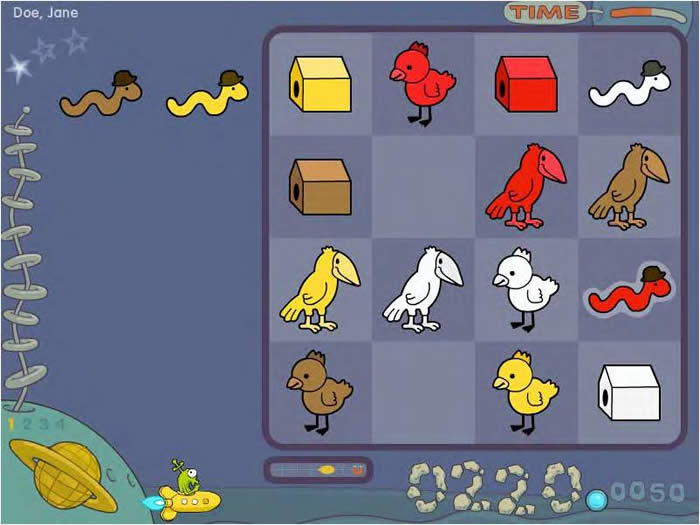
\includegraphics[scale = .4]{Chapters/related_work_img/FastForWord_Cosmic_Reader.jpg}
    \caption{Fast ForWord - Cosmic Reader}
    \label{fig:fastforword}
\end{figure}
% https://www.gemmlearning.com/programs/fast-forword/

% https://www.apa.org/topics/learning-memory/dyslexia-video-games
% https://www.scilearn.com/ - Game Site

% https://www.apa.org/topics/learning-memory/dyslexia-video-games
% https://www.unicef.org/parenting/child-care/10-playful-educational-activities-children-disabilities
% https://www.parentcircle.com/games-and-activities-for-special-needs-and-autistic-children/article
% https://www.commonsensemedia.org/articles/5-ways-video-games-can-help-kids-with-disabilities
% https://parentingpod.com/dyslexia-activities/